\documentclass[12pt]{article}
\usepackage[letterpaper, margin=1in]{geometry}
\usepackage{graphicx}
\usepackage{subcaption}
\graphicspath{{./Figures/}}
\usepackage{hyperref}
\usepackage{parskip}
\usepackage{amsmath}
%\allowdisplaybreaks % in case equations need to be broken across lines, probably should use align* with \stepcounter{equation}\tag{\theequation}\label{eq:7omegan} for equation numbering

\title{ELECENG 3CL4 Lab 2 Report}
\author{
    Aaron Pinto \\
    pintoa9 \\
    L02
    \and
    Raeed Hassan \\
    hassam41 \\
    L02
}

\begin{document}

\maketitle
\clearpage

\section*{Member Contributions}
Both group members contributed an even amount to both the exercises and the report. Both members went through the exercises together and contributed to all sections of the report.

\section*{Objective} % This is the brief description of the objective of the lab
The objective of this lab was to identify the plant model of a marginally-stable servomotor for the subsequent experiments.

\clearpage
\setcounter{section}{2}
\section{Perform Closed Loop Identification}
\subsection{Experiment 1: Time Domain Identification}
% iii) ran sim
With a default proportional gain of 1, we observed some small non-linear effects when the servo motor slows down, where the servo angle plot went from a curve to a line at the end of the movements. This is visible in the graph shown below.
%SHOW THE GRAPH HERE OF K = 1
% iv) K = 2
When we increased the proportional gain to 2, we observed that the small non-linear effects shown above were greatly reduced. Consequently, the overshoot of the servo motor increased as a result of the P-gain increase. The motor voltage and servo angle plots can be seen in Figure~\ref{fig:exp1}.
\begin{figure}[h!]
    \centering
    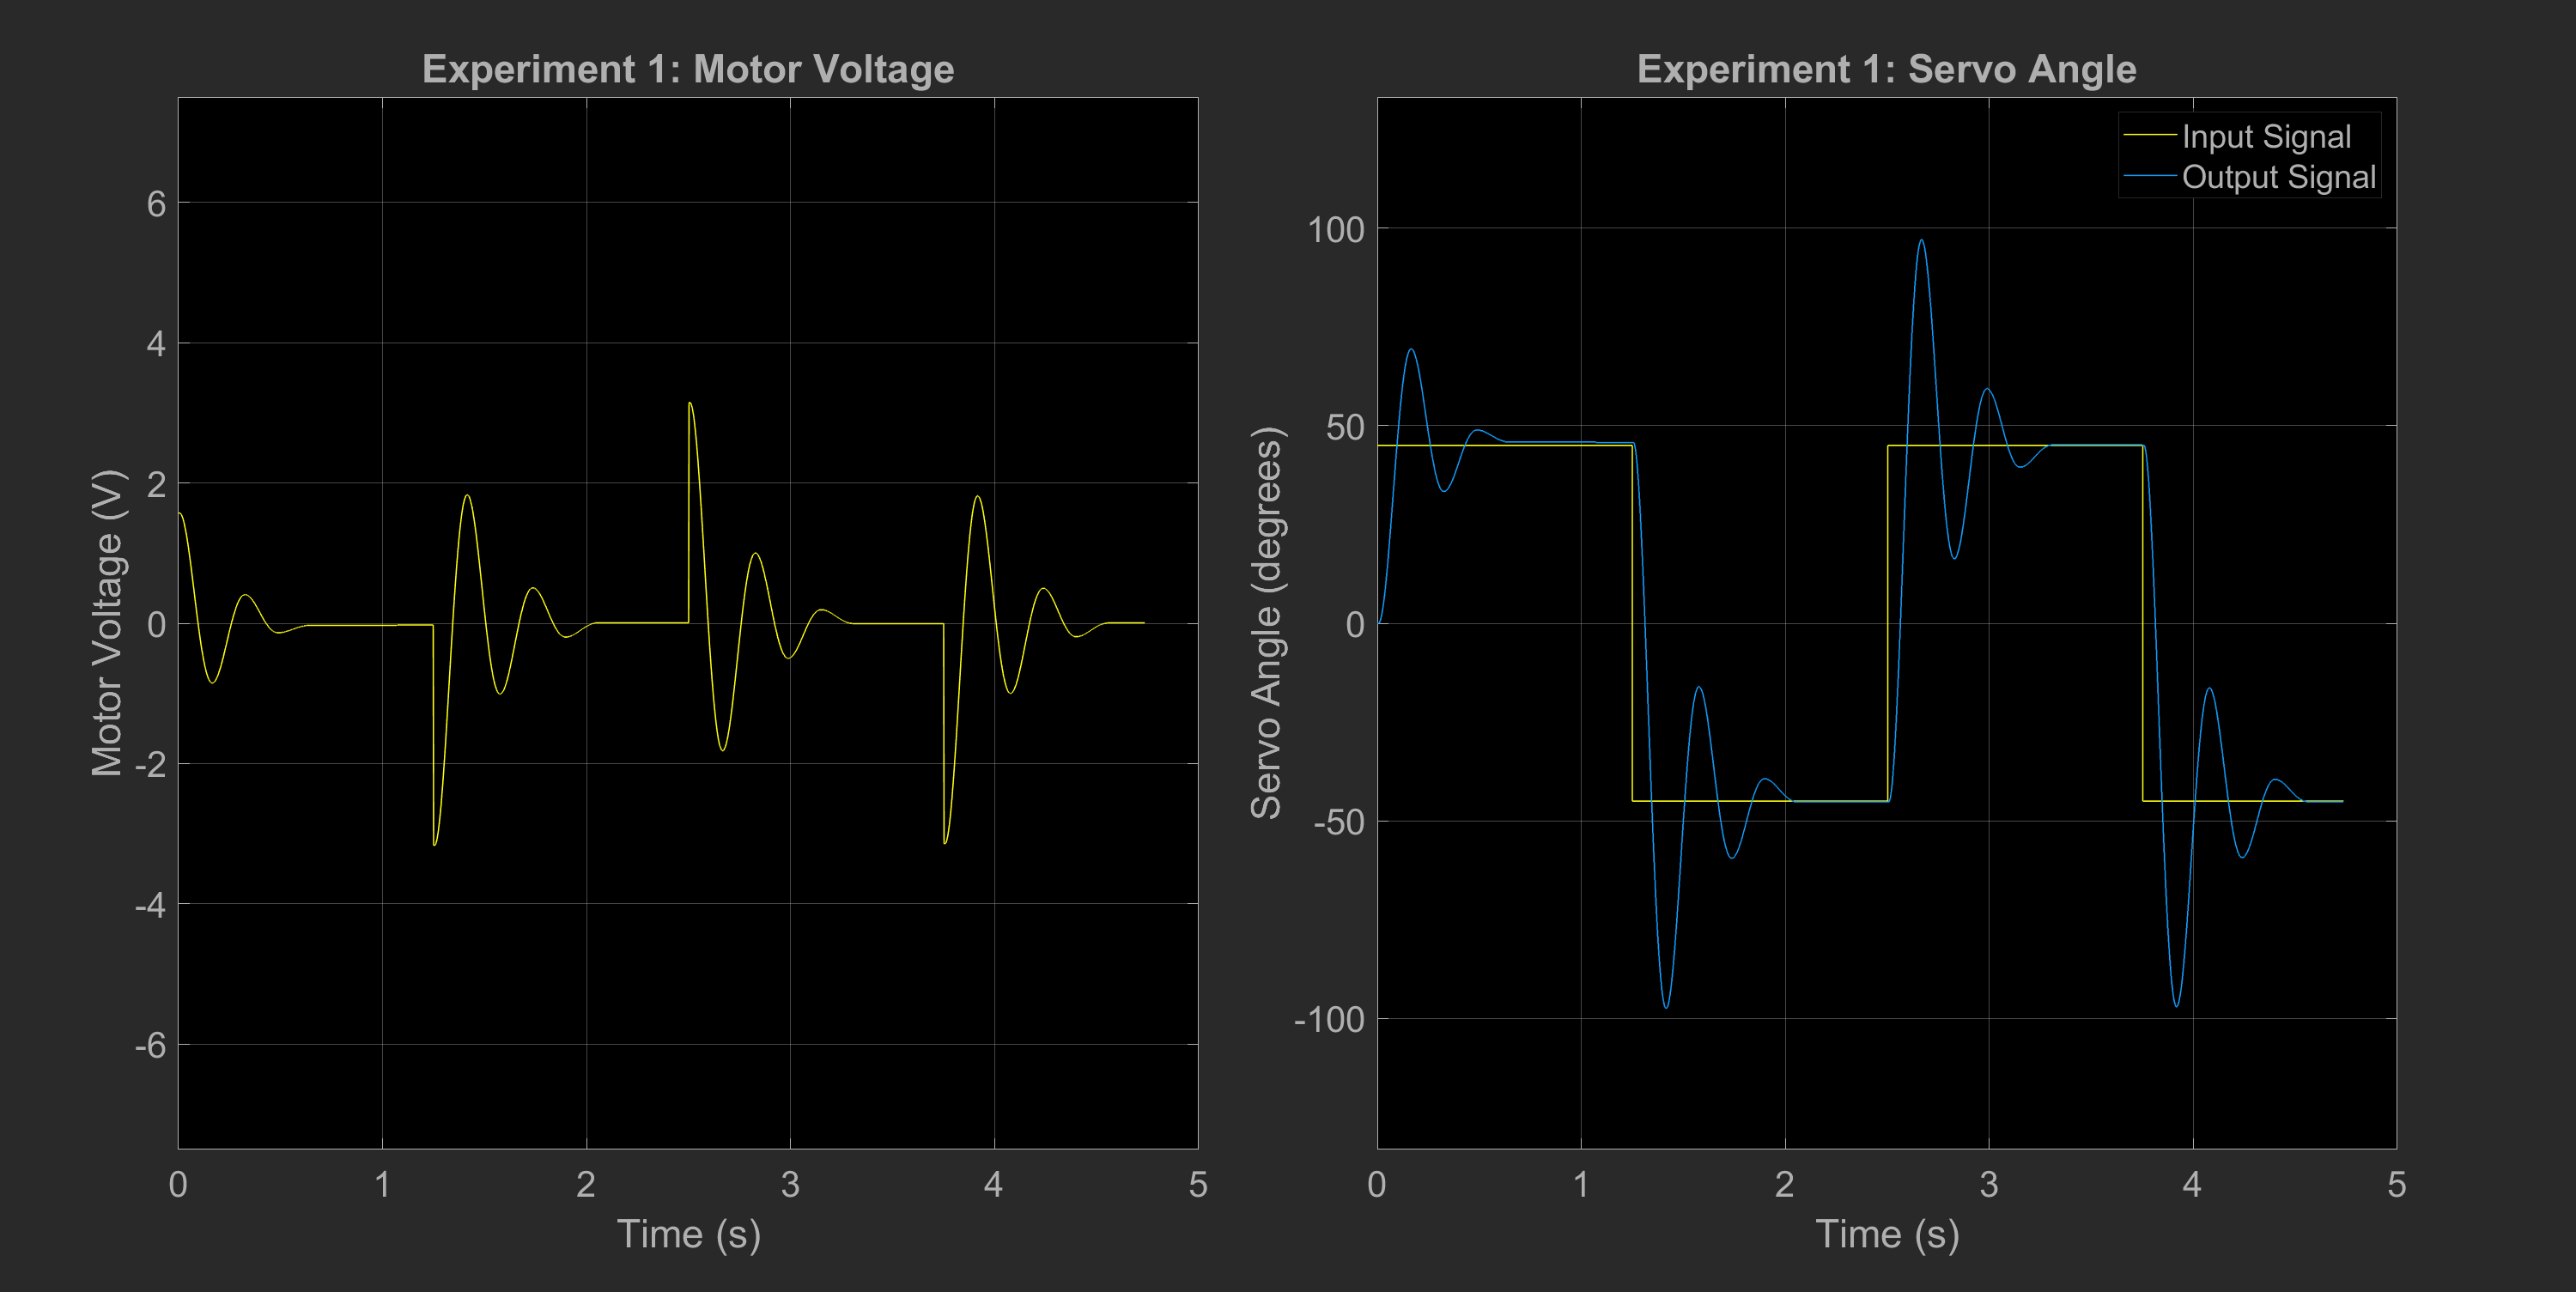
\includegraphics[width=\textwidth]{exp1}
    \caption{\label{fig:exp1}Motor Voltage and Servo Angle for Time Domain Identification}
\end{figure}

% v) measure height of first overshoot peak, time of first overshoot peak
% vi) measure the stuff
% vii) measure time difference from edge to time of first peak
% viii) record measurements
The amplitude of the input square wave was 45 degrees. The switching time was determined to be negligible and assumed to be 0.

To measure the height and time of the first overshoot peak, we use the "Peak Finder" tool in the scopes. The tool determines the peaks in the plots and states the value of the peak and the time it occurs. The height of the first overshoot peak was 69.43 degrees, and the time of the first overshoot peak was 0.162 seconds.
% ix) use measurements to calculate motor parameters
We can use the recorded measurements to determine the percent overshoot $P.O.$ and the peak time $T_p$.
\begin{equation*}
\begin{aligned}[b]
    P.O. &= 100\left(\frac{69.43}{45}\right) - 100 & T_p &= 0.162 \\
    &\approx 54.3\%
\end{aligned}
\end{equation*}
We can determine $\zeta$ and $\omega_n$ by using the equations derived in the prelab which relate them to $P.O.$ and $T_p$.
\begin{equation*}
\begin{aligned}
    \zeta &= \frac{-\log\left(\frac{P.O.}{100}\right)}{\sqrt{\pi^2 + \left(\log\left(\frac{P.O.}{100}\right)\right)^2}} & \omega_n &= \frac{\pi}{T_p\sqrt{1-\zeta^2}} \\
    &= 0.191 & &= 19.756
\end{aligned}
\end{equation*}
We can determine the motor parameters $A$ and $\tau_m$ by using the equations derived in the prelab which relate them to $\zeta$ and $\omega_n$.
\begin{equation} \label{fig:exp1calc}
\begin{aligned}[b]
    A &= \frac{\omega_n / 2\zeta}{K} & \tau_m &= \frac{1}{2\omega_n\zeta} \\
    &= 25.877 & &= 0.133
\end{aligned}
\end{equation}

The values of $A$ and $\tau_m$ were determined to be 25.877 and 0.133 in Equation~\ref{fig:exp1calc}.

\subsection{Experiment 2: Frequency Domain Identification}
% i) verify that the choice of K = 2 gives a value of zeta that leads to a reasonable peak in Fig 3.
To verify that the choice of K = 2 lead to a reasonable peak shown in Figure 3 of the lab document, we calculated that our $\zeta$ was 0.191, and from Figure 3 in the lab document we observed that it gave us a peak of approximately 8 dB, which is large enough that we could easily identify the peak.

% vi) observe at 0.5 hz; small delay, some non-linear effects at direction change
Starting at 0.5 Hz, we observed essentially the same signal magnitude between the input and servo angle signals, and a small delay in the angle signal relative to the input, both of which are as expected from the magnitude and phase response in the bode plot (Figure 3 in the lab document). There were also some small non-linearities at the tips of the angle signal, where the motor changed direction, which meant that the output (shown below) was not quite sinusoidal. The motor voltage and servo angle plots at 0.5 Hz can be seen in Figure~\ref{fig:exp2_0.5}.
\begin{figure}[h!]
    \centering
    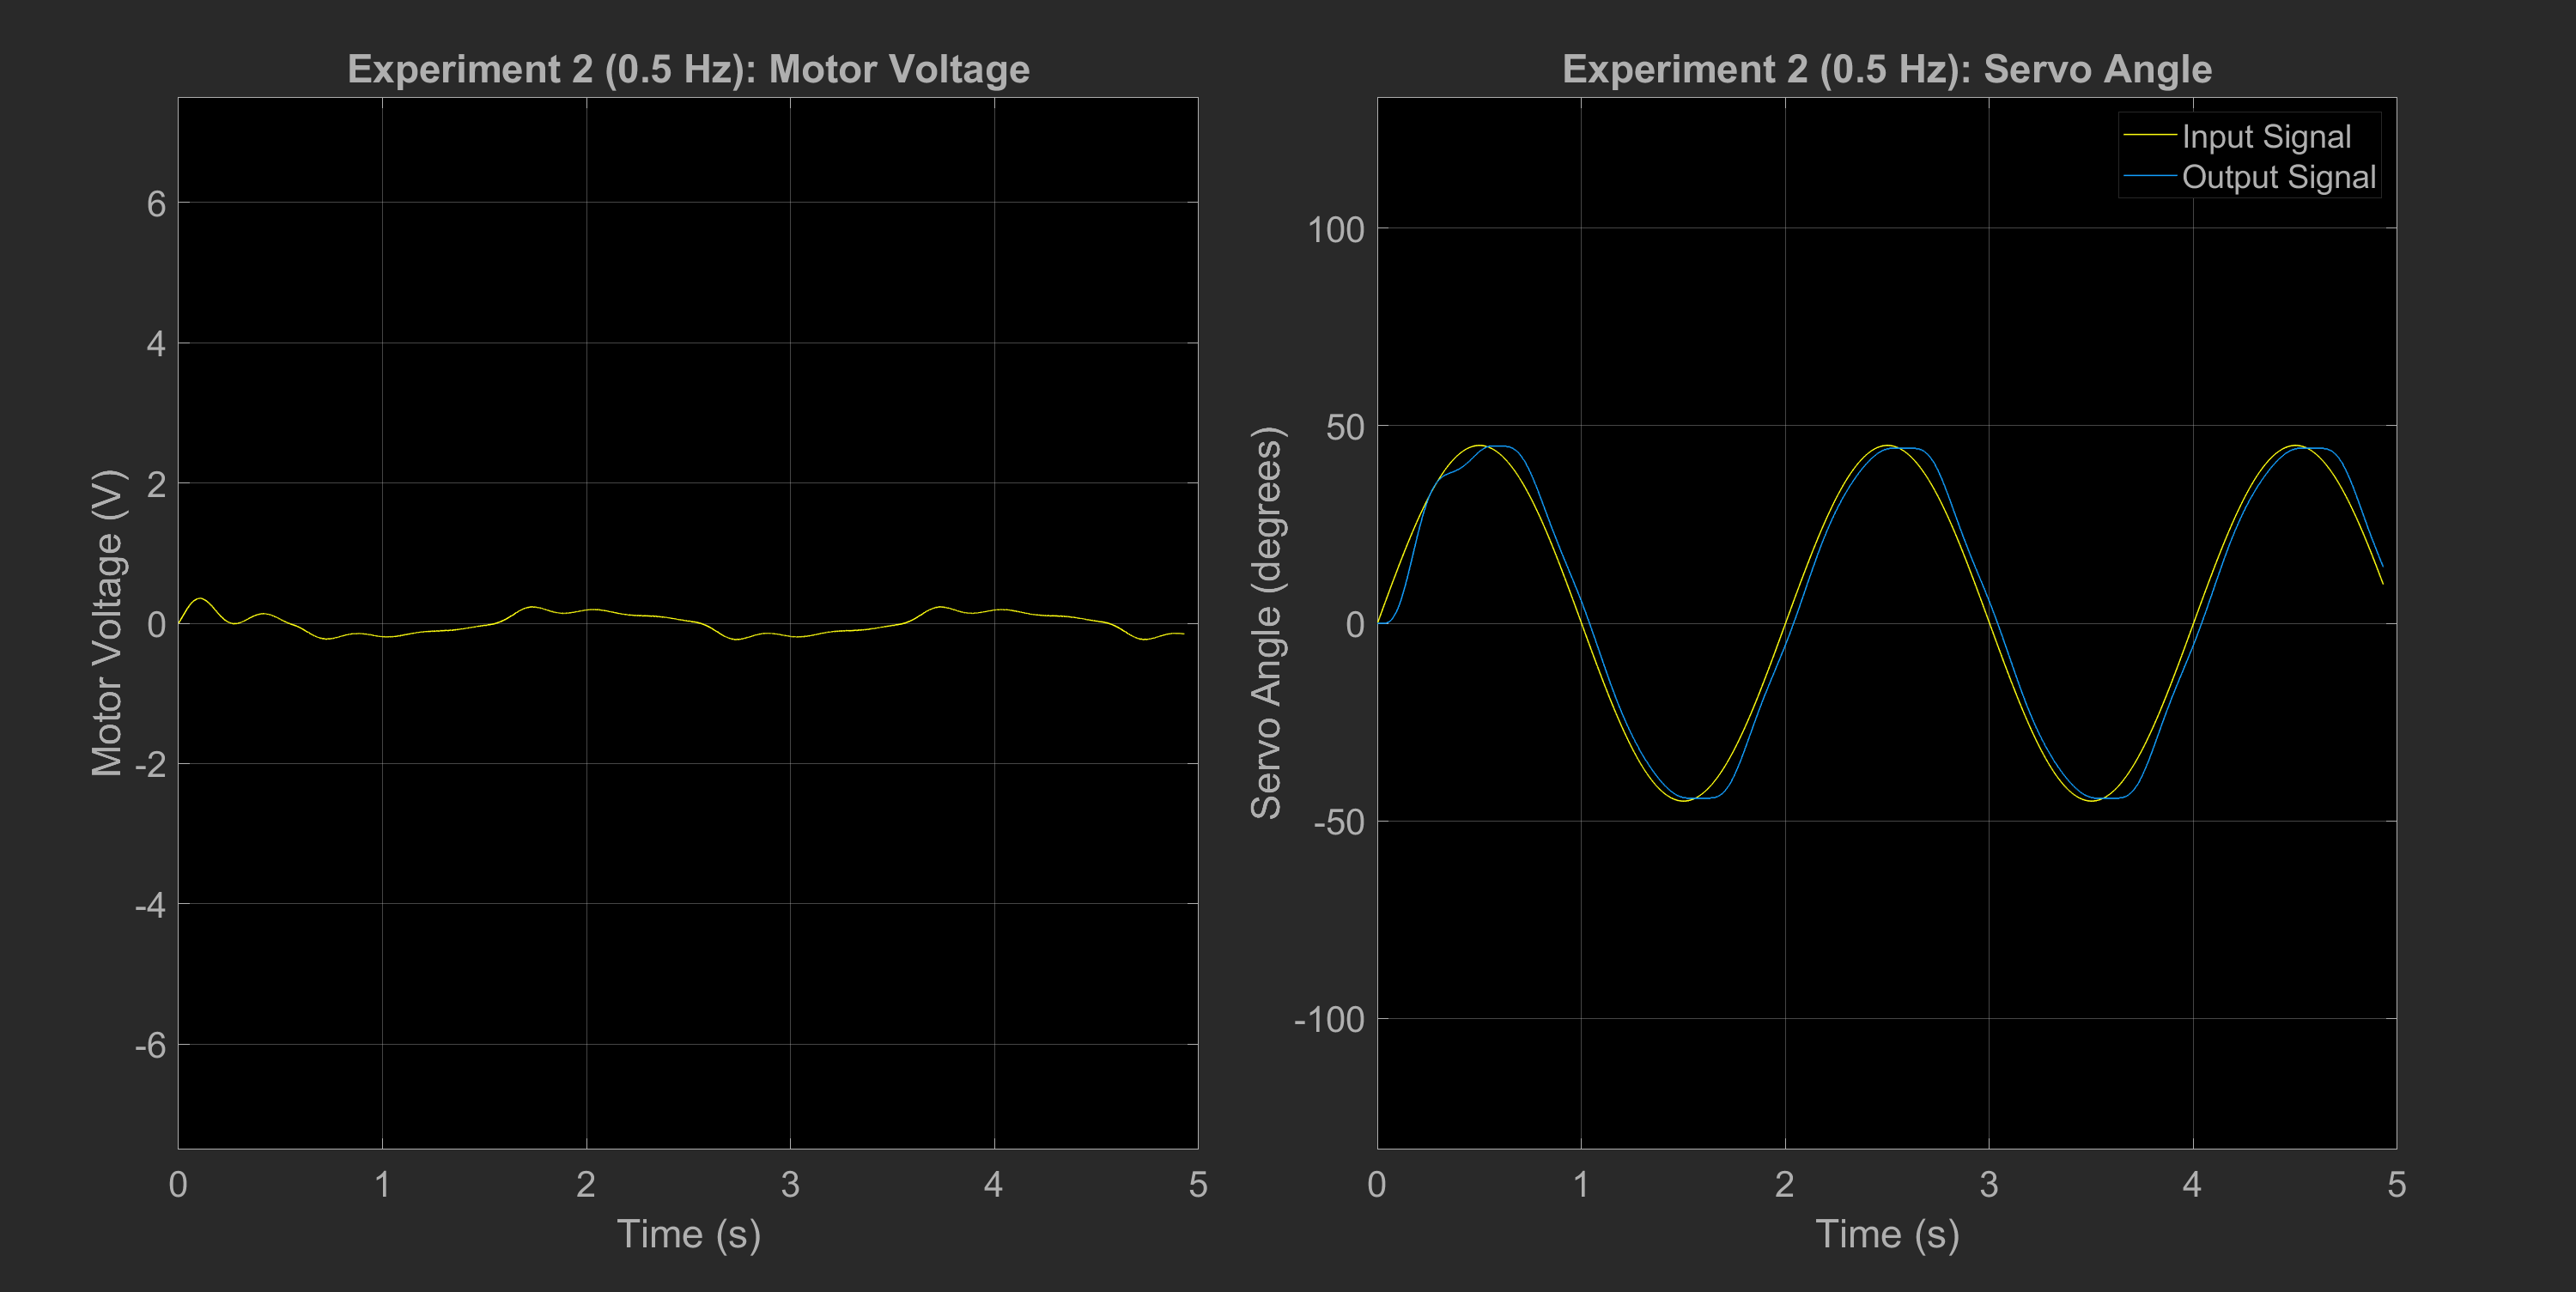
\includegraphics[width=0.87\textwidth]{exp2_0.5}
    \caption{\label{fig:exp2_0.5}Motor Voltage and Servo Angle for 0.5 Hz Input Signal}
\end{figure}

% vii) 1 hz; slightly greater gain, slight longer delay, non-linear effects diminished
Increasing the input frequency to 1 Hz slightly increased both the gain and delay of the system, like in the bode plot. The non-linear effects were reduced but still present. The motor voltage and servo angle plots at 1 Hz can be seen in Figure~\ref{fig:exp2_1}.
\begin{figure}[h!]
    \centering
    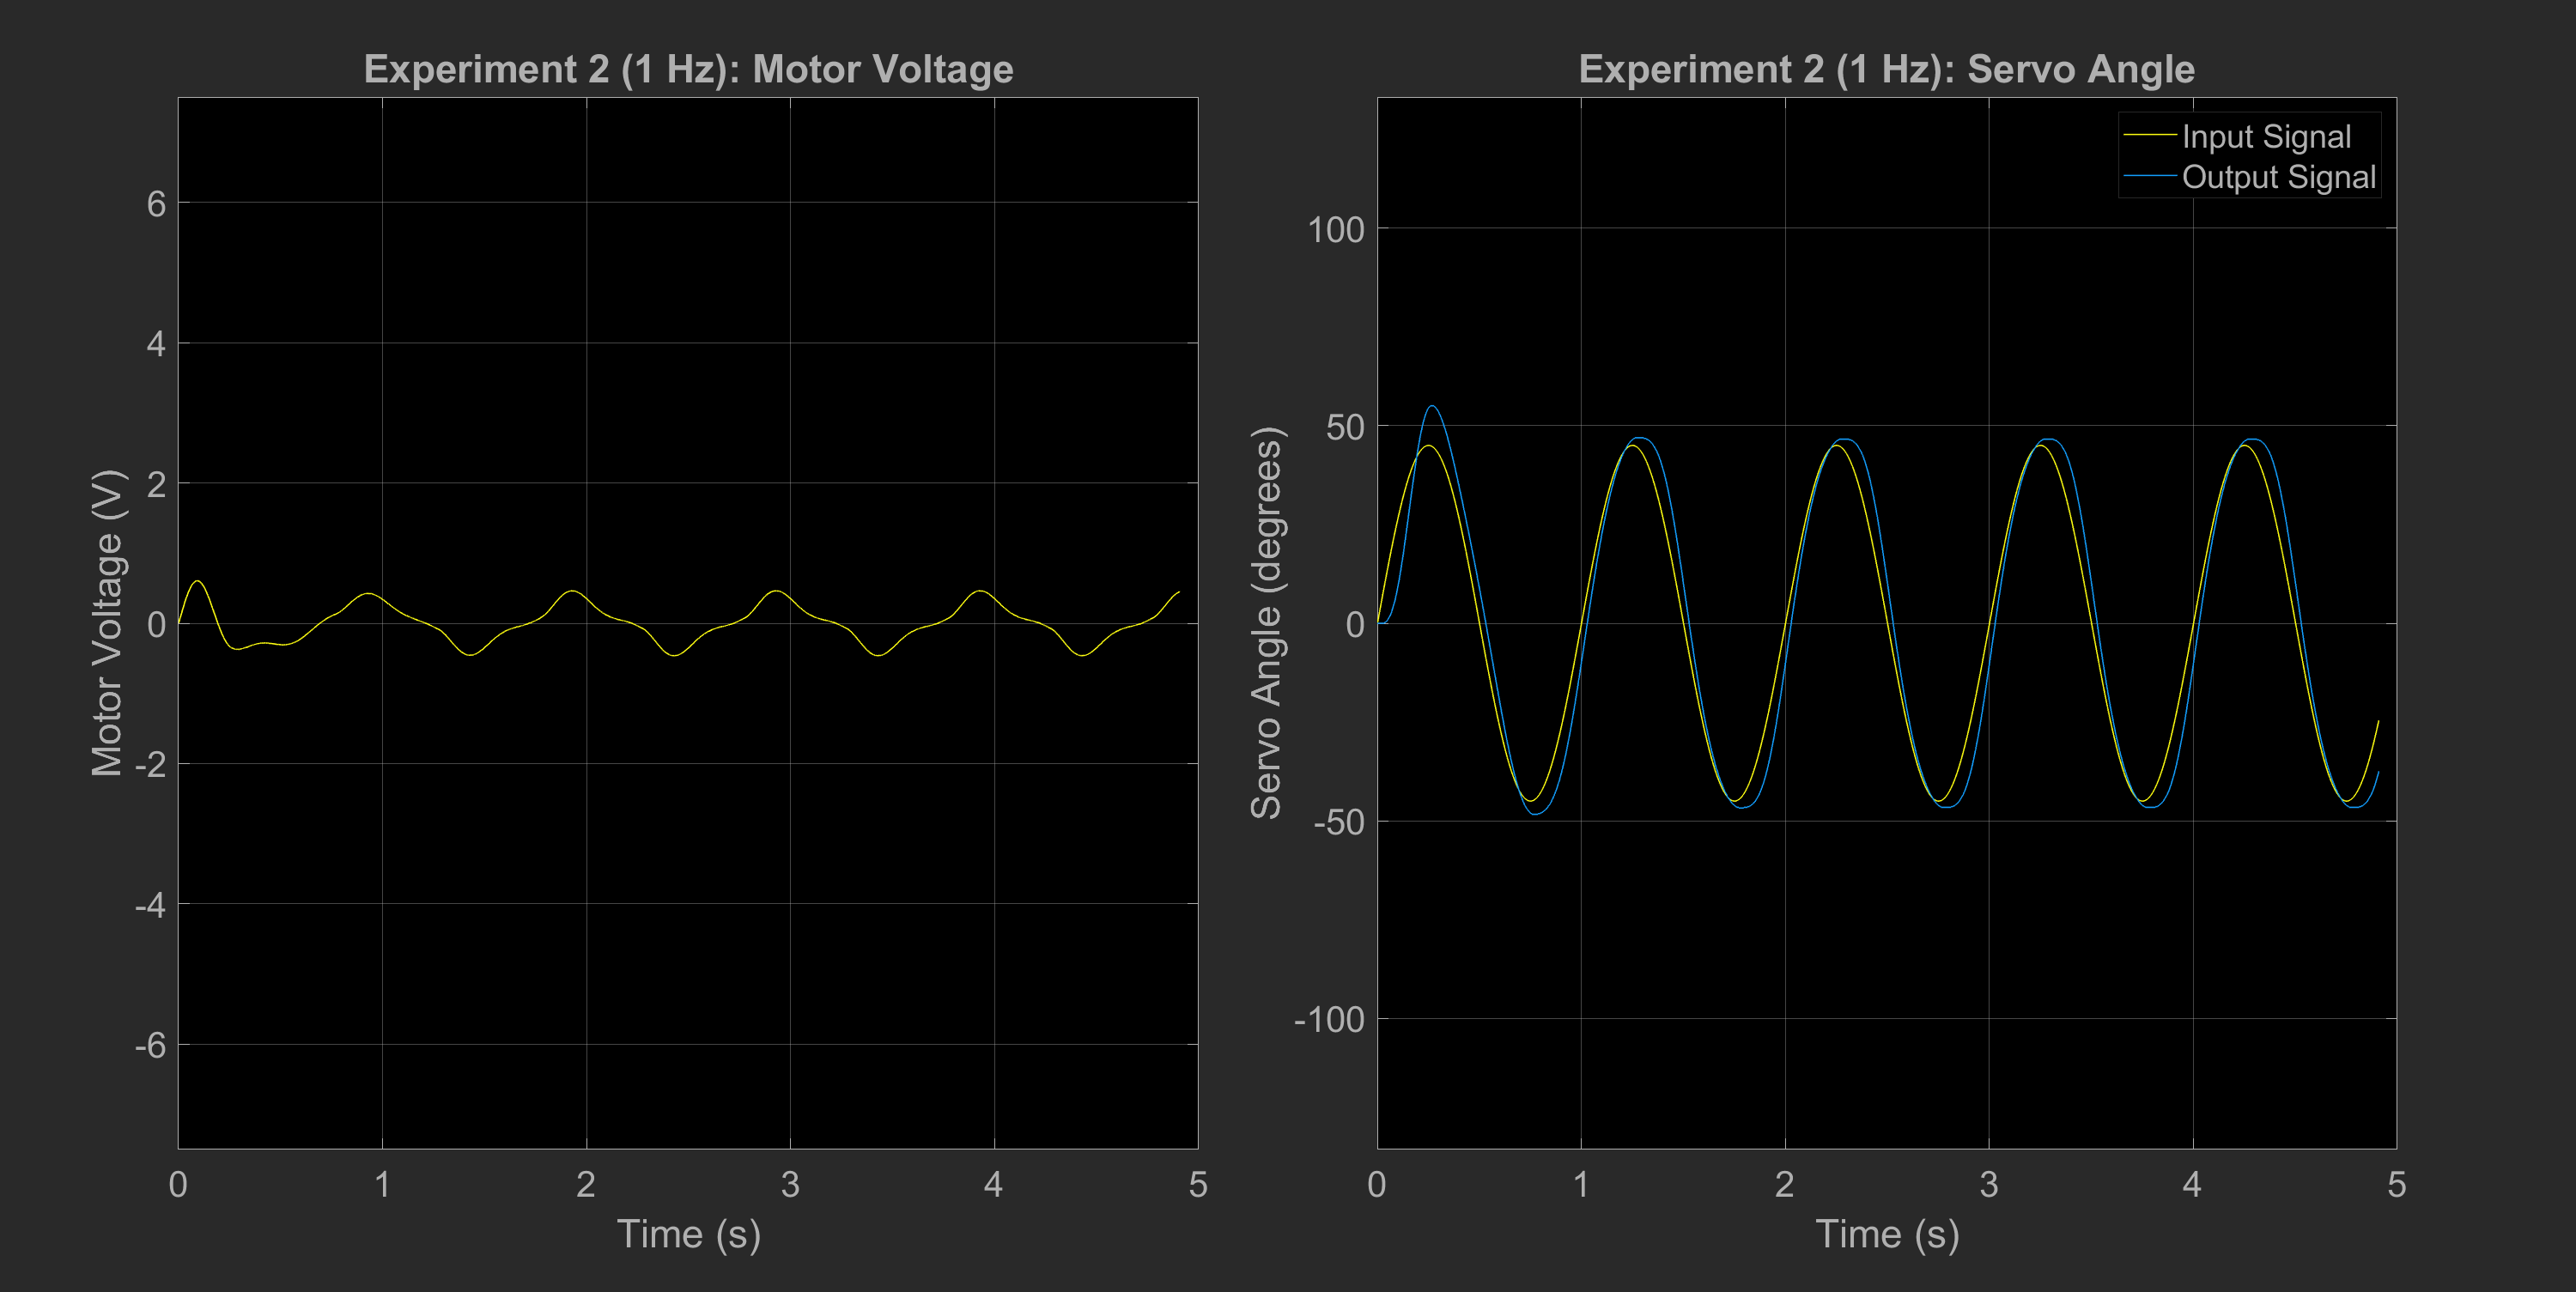
\includegraphics[width=0.87\textwidth]{exp2_1}
    \caption{\label{fig:exp2_1}Motor Voltage and Servo Angle for 1 Hz Input Signal}
\end{figure}

% viii) 2 hz; gain signif greater, moderate delay, non-linear effects negligible
At 2 Hz, the gain was much greater than 1 and the delay was much larger as well, which is as expected as we move further right on the bode plot. The non-linear effects were completely negligible at this point. The motor voltage and servo angle plots at 2 Hz can be seen in Figure~\ref{fig:exp2_2}.
\begin{figure}[h!]
    \centering
    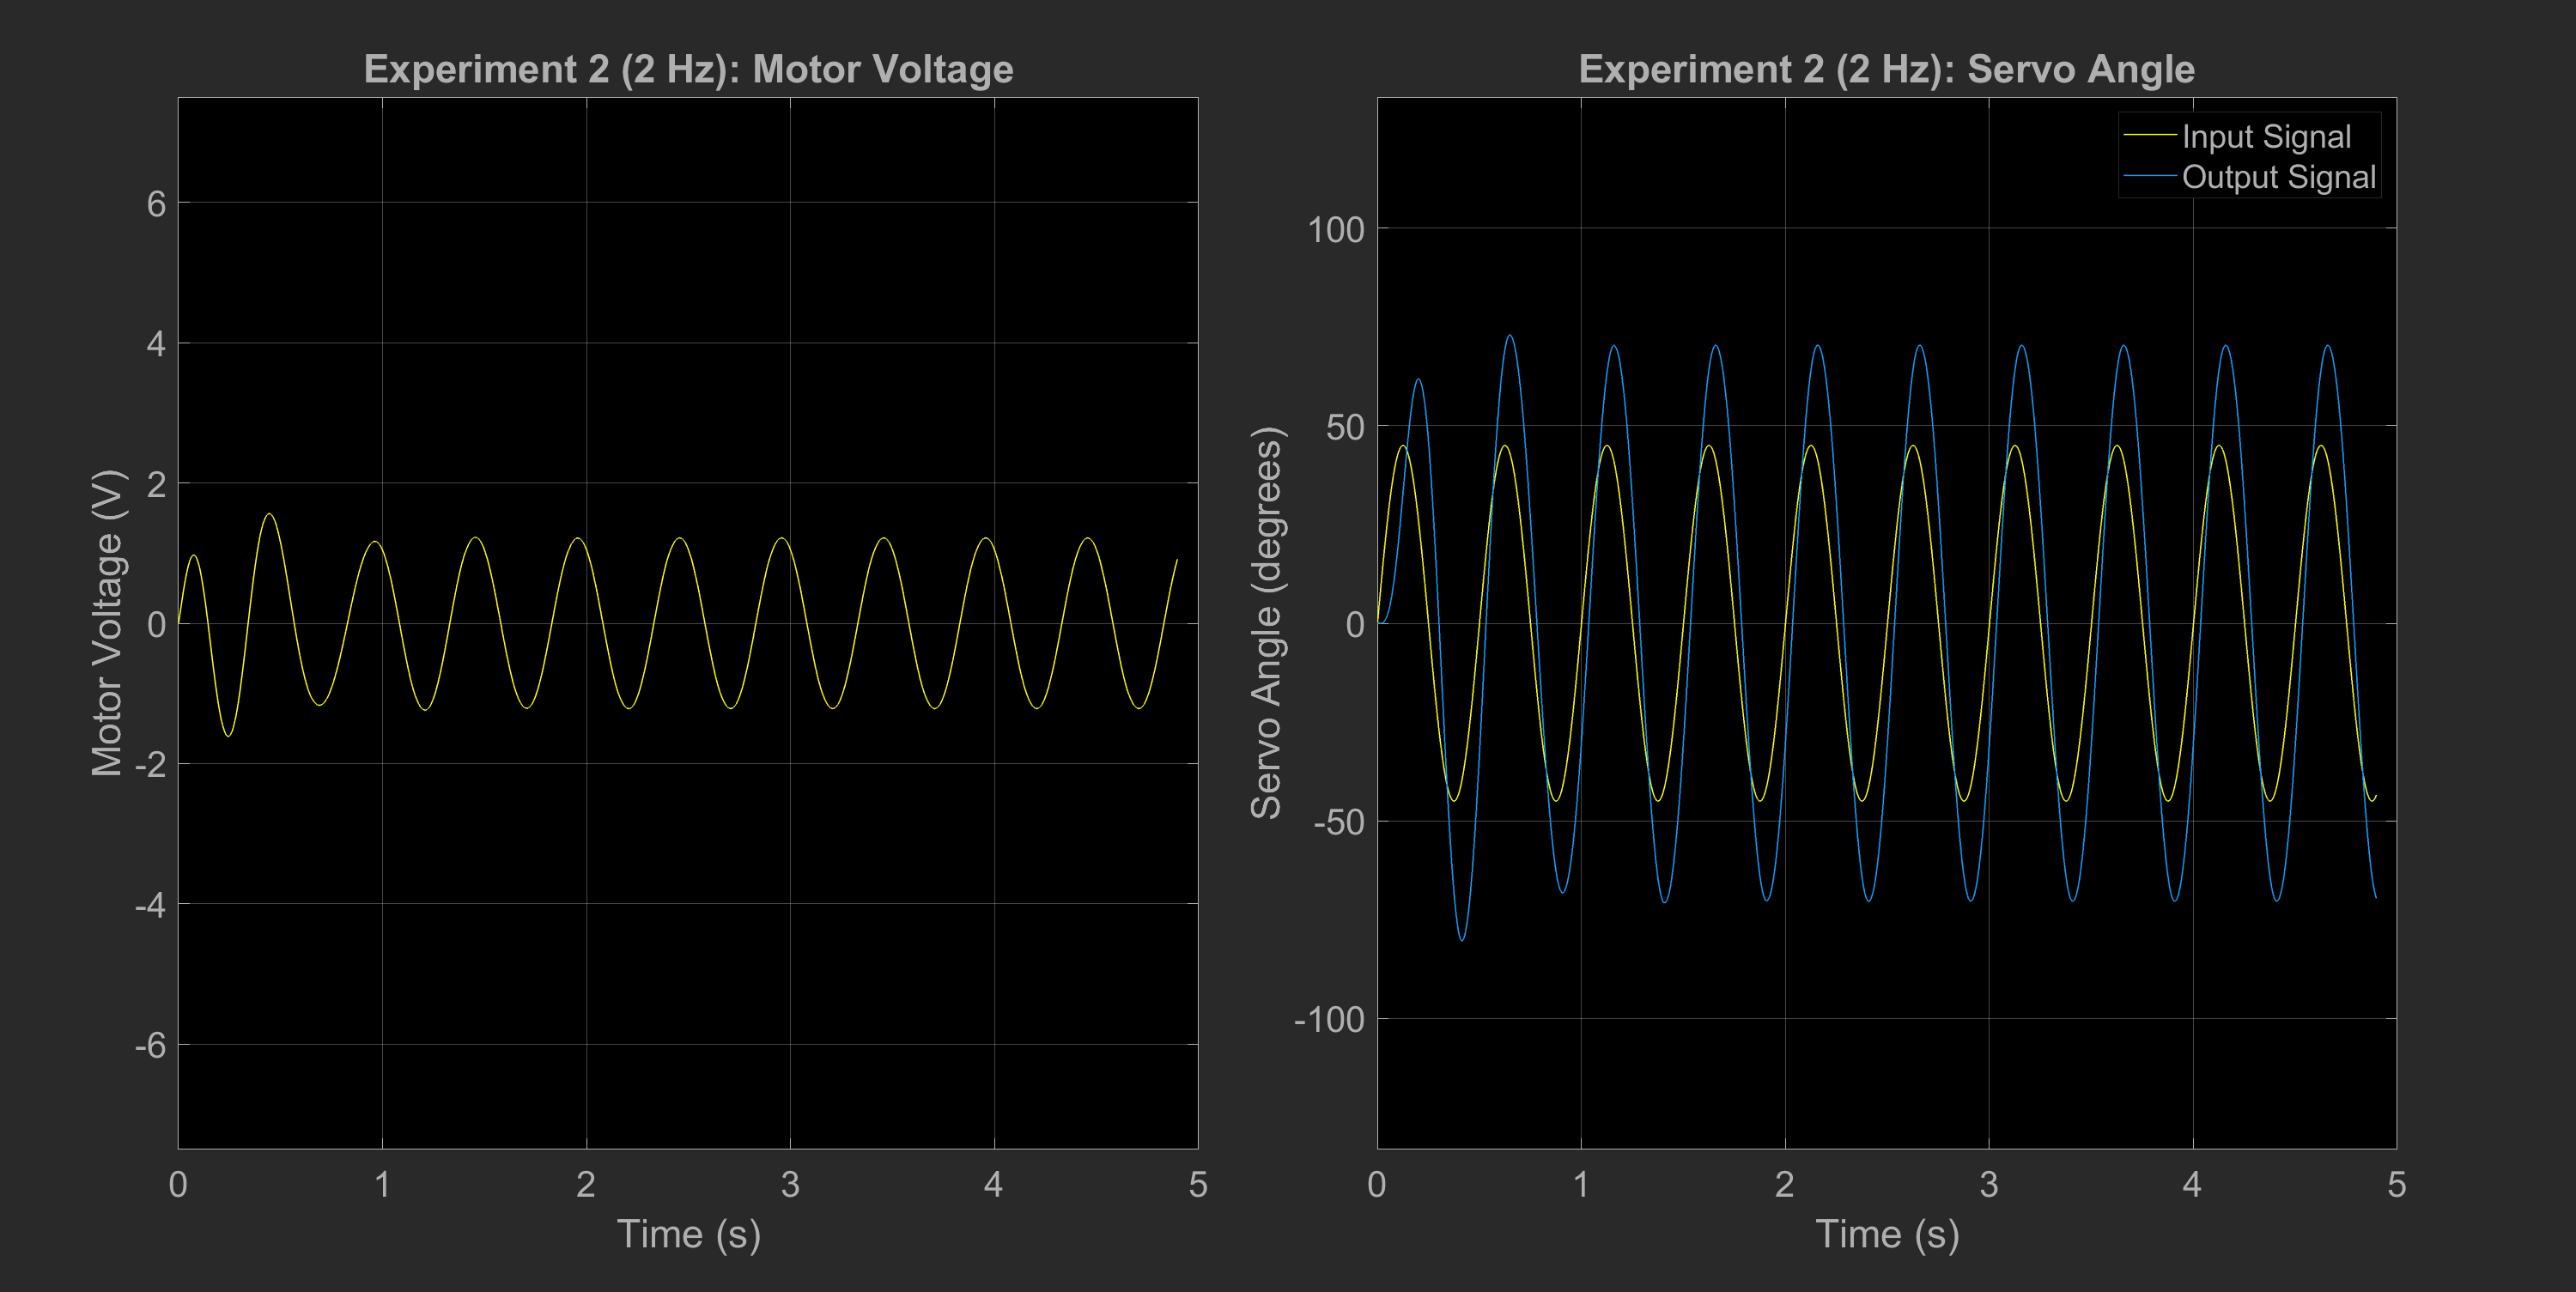
\includegraphics[width=0.87\textwidth]{exp2_2}
    \caption{\label{fig:exp2_2}Motor Voltage and Servo Angle for 2 Hz Input Signal}
\end{figure}

% ix) 3 hz; gain signif greater, signifc delay, non-linear effects negligible
At 3 Hz, the gain increased significantly as the frequency likely corresponds to the region around the peak of the bode magnitude plot. The phase delay is now significant, as the frequency enters the region of bode phase plot where there is a step decrease in the phase. The motor voltage and servo angle plots at 3 Hz can be seen in Figure~\ref{fig:exp2_3}.
\begin{figure}[h!]
    \centering
    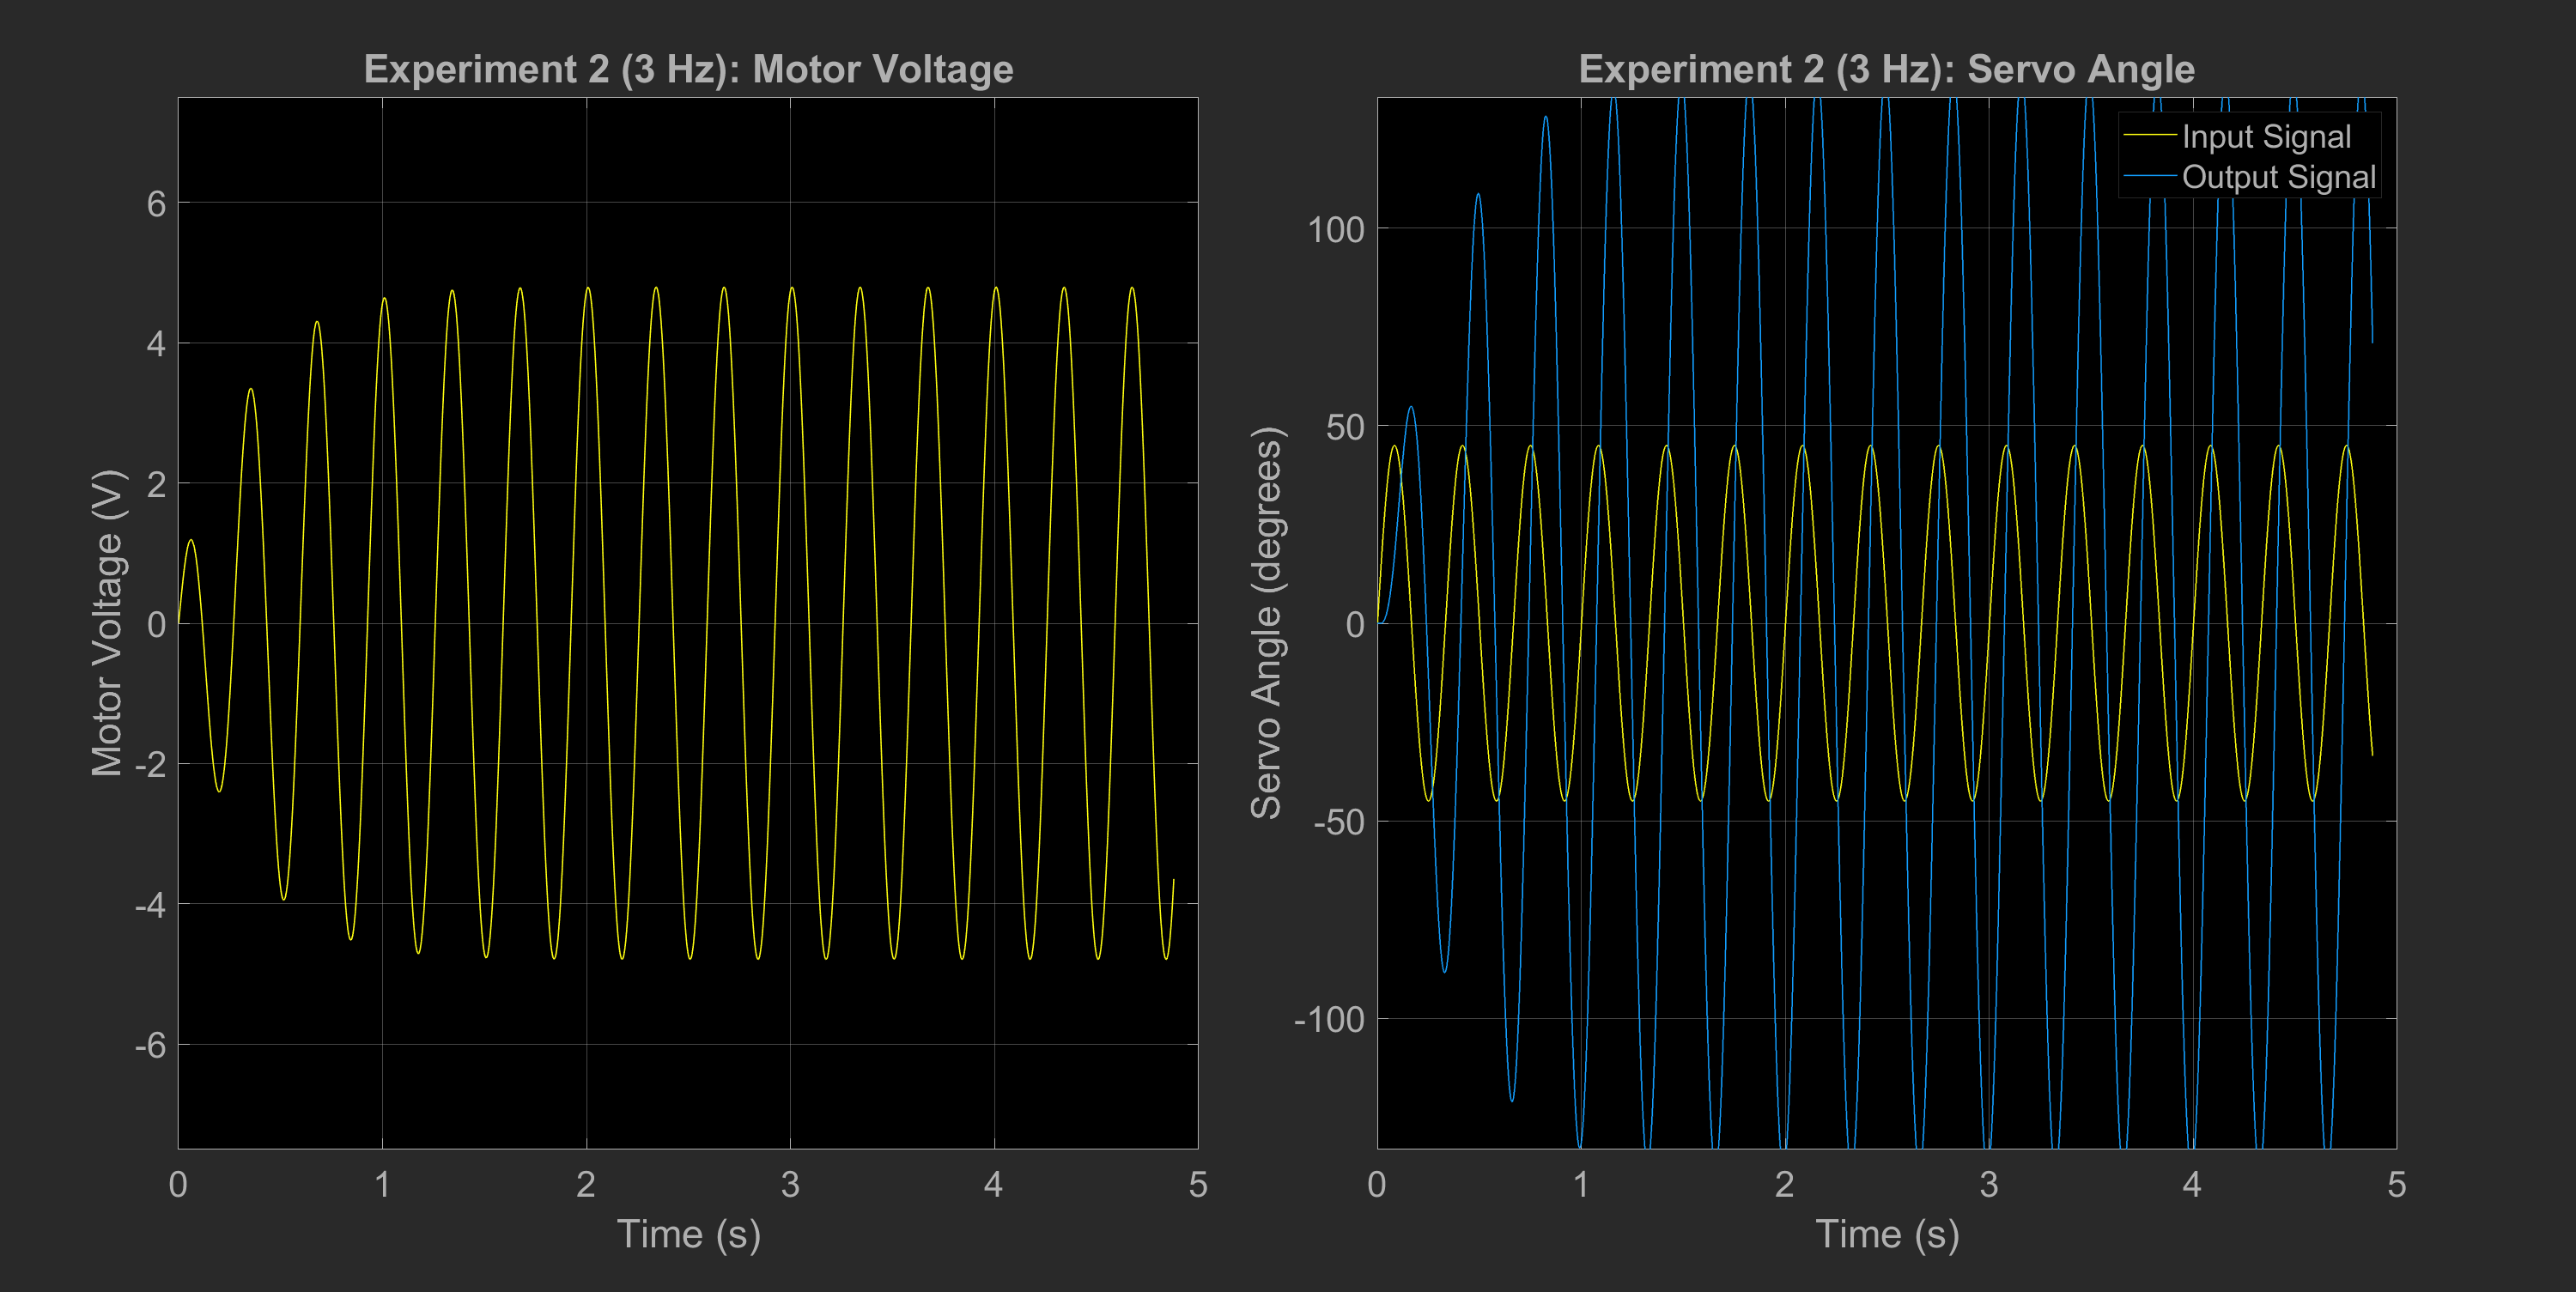
\includegraphics[width=0.87\textwidth]{exp2_3}
    \caption{\label{fig:exp2_3}Motor Voltage and Servo Angle for 3 Hz Input Signal}
\end{figure}

% x) 4 hz; gain smaller than 3 hz, output almost completely out of phase w/ input
At 4 Hz, the gain decreases which matches the behaviour of the bode magnitude plot, where the magnitude peaks at a certain frequency before beginning to decrease. The output signal is also completely out of phase with the input by this point, which is around where the bode phase plot begins to plateau around -180 degrees. The motor voltage and servo angle plots at 4 Hz can be seen in Figure~\ref{fig:exp2_4}.
\begin{figure}[h!]
    \centering
    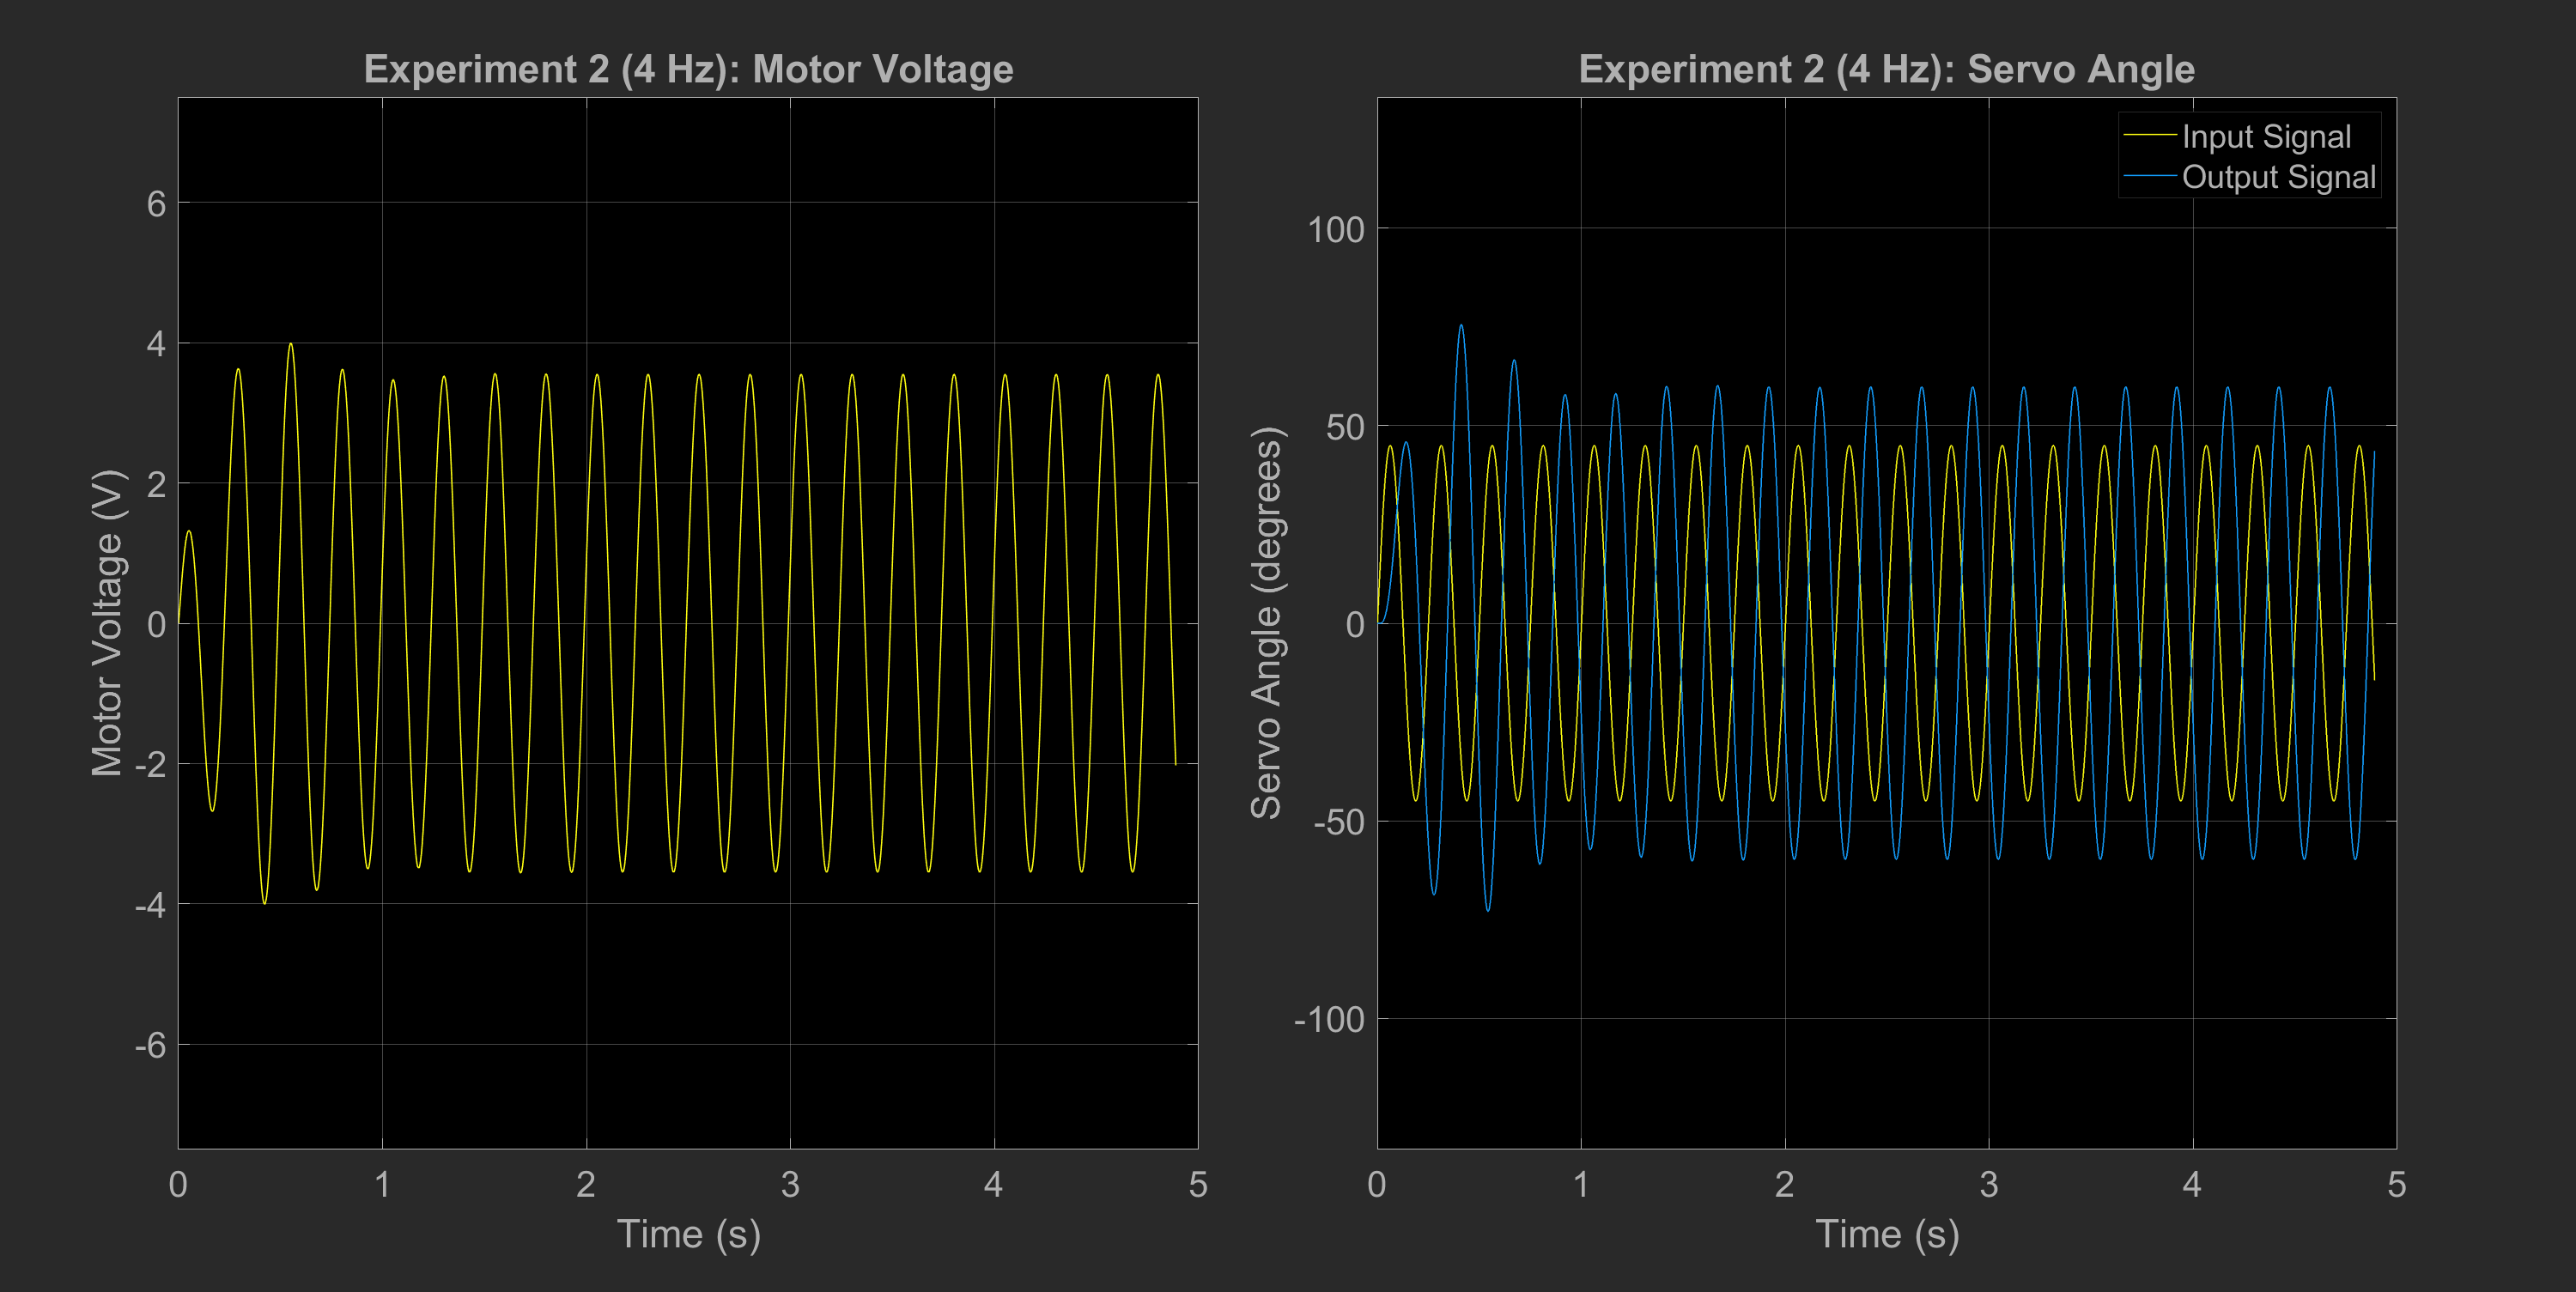
\includegraphics[width=0.87\textwidth]{exp2_4}
    \caption{\label{fig:exp2_4}Motor Voltage and Servo Angle for 4 Hz Input Signal}
\end{figure}

% xi) 5 hz; 
At 5 Hz, the gain decreases even further, falling below 0 dB and attenuating the output signal, putting the frequency in the region where the bode magnitude plot is decreasing at a steady rate. The phase delay is around the same as it was at 4 Hz. The motor voltage and servo angle plots at 5 Hz can be seen in Figure~\ref{fig:exp2_5}.
\begin{figure}[h!]
    \centering
    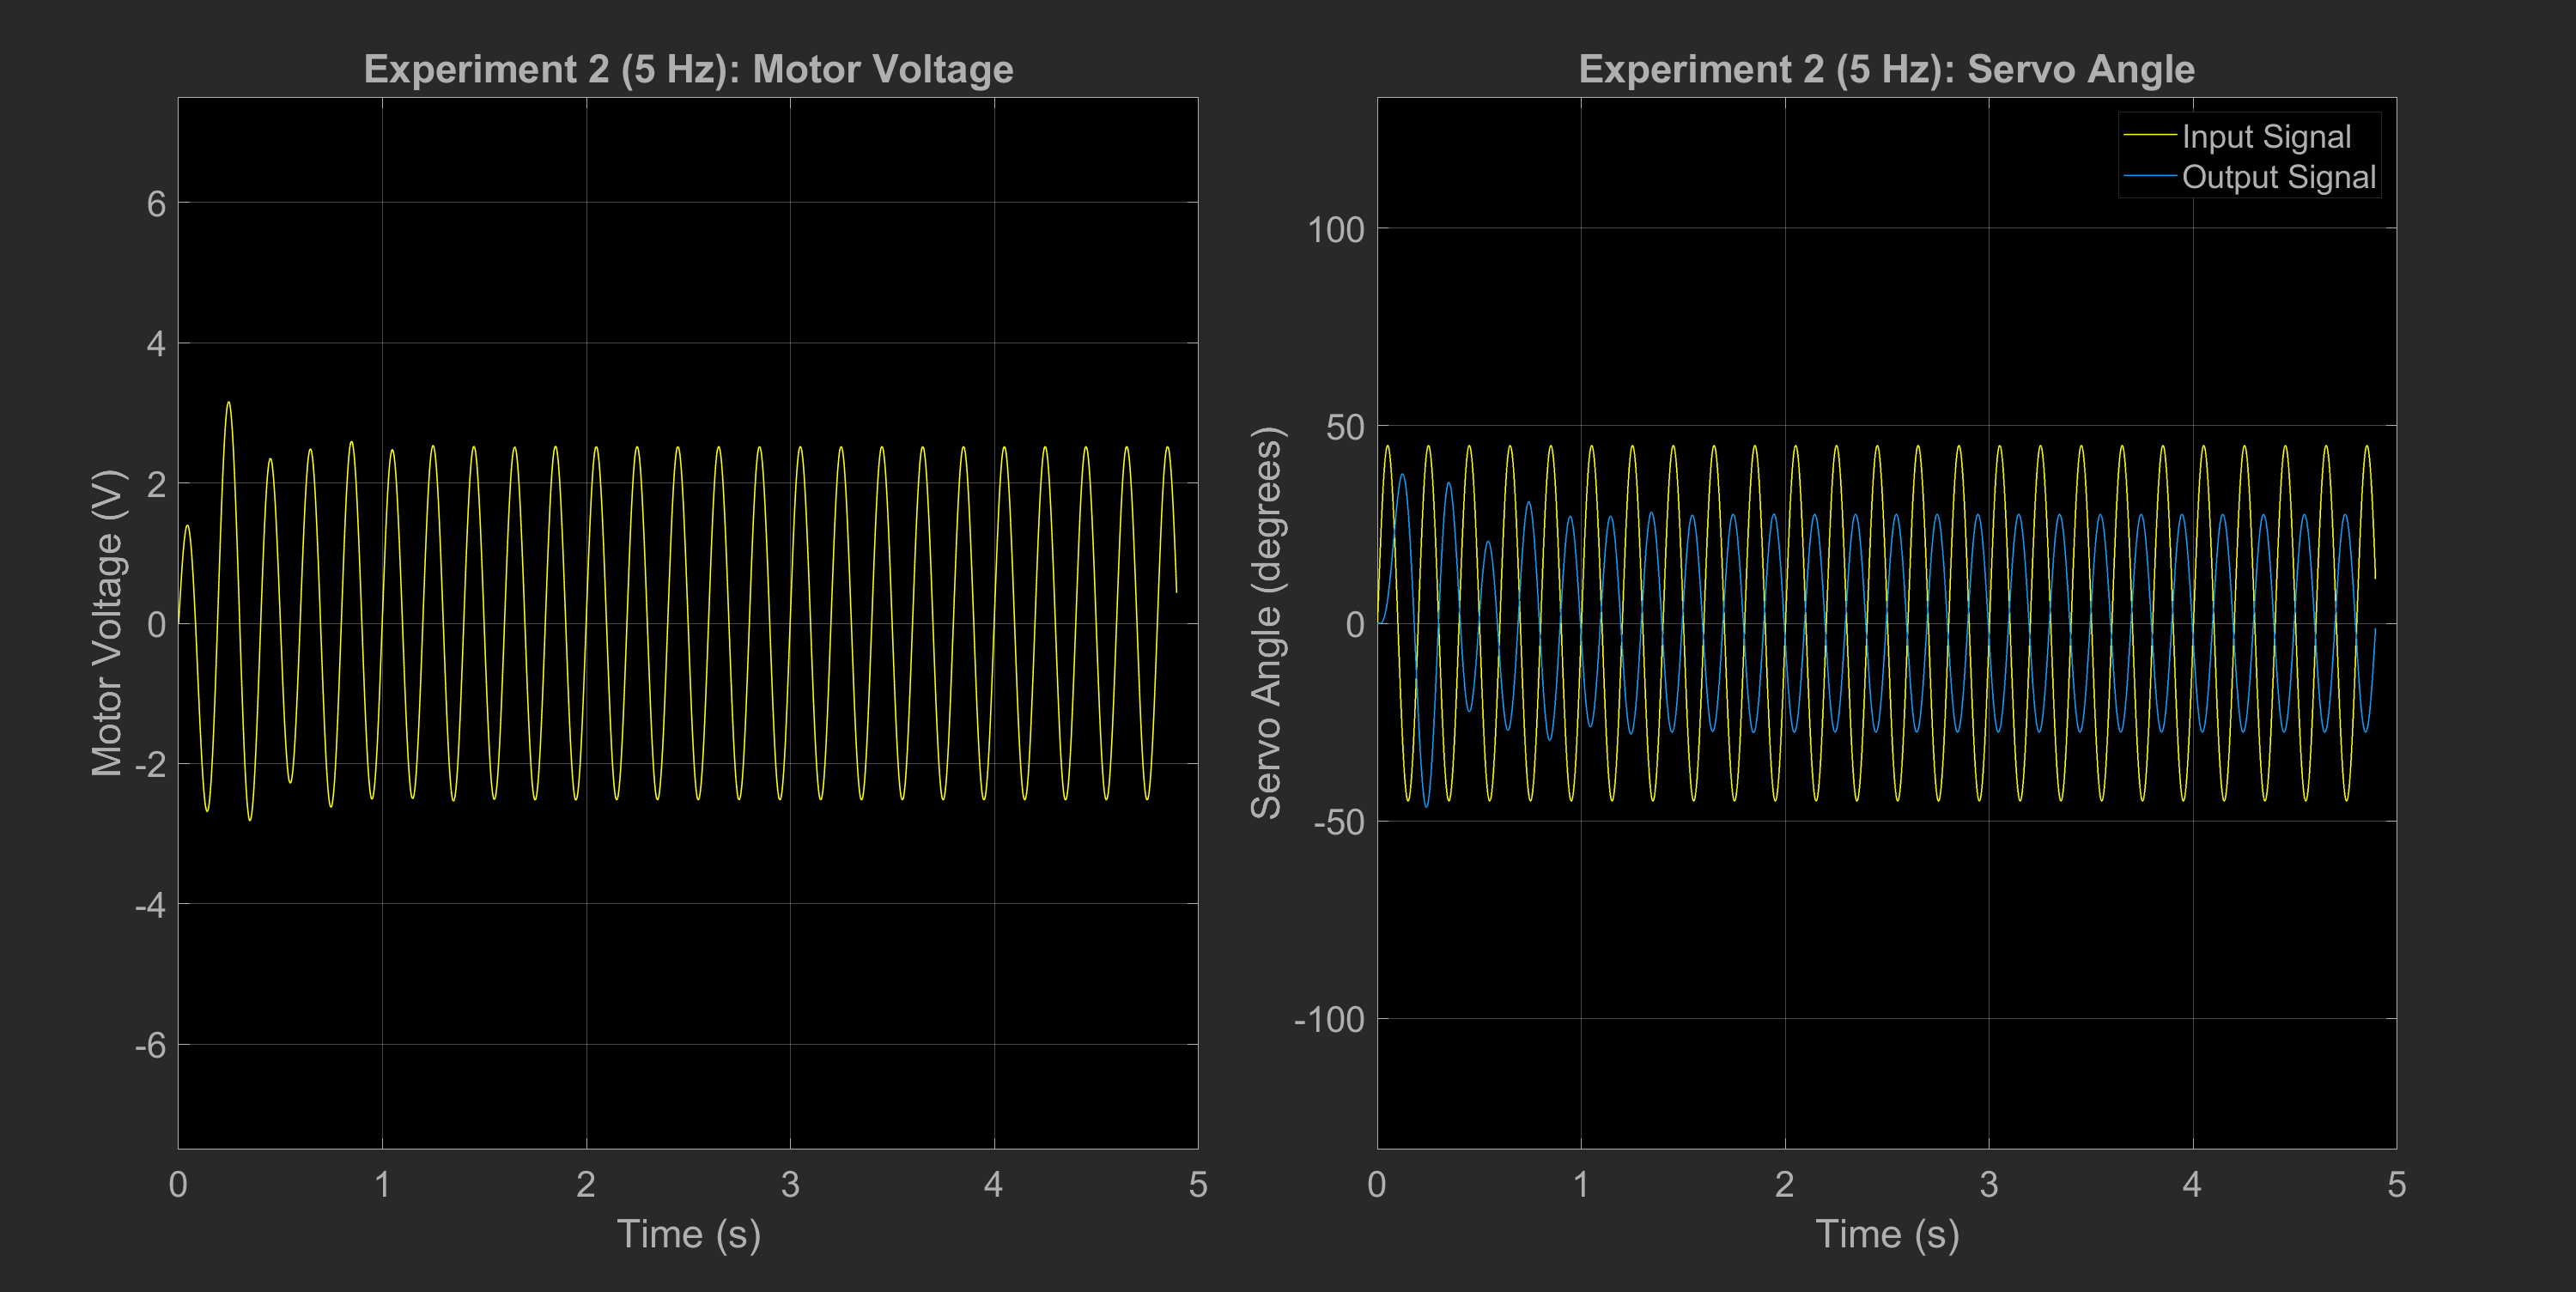
\includegraphics[width=0.87\textwidth]{exp2_5}
    \caption{\label{fig:exp2_5}Motor Voltage and Servo Angle for 5 Hz Input Signal}
\end{figure}

% xii) 6 hz;
At 6 Hz, the gain continues to decrease while the phase delay remains around the same, matching the behaviour that we expect from the bode plot. The motor voltage and servo angle plots at 6 Hz can be seen in Figure~\ref{fig:exp2_6}.
\begin{figure}[h!]
    \centering
    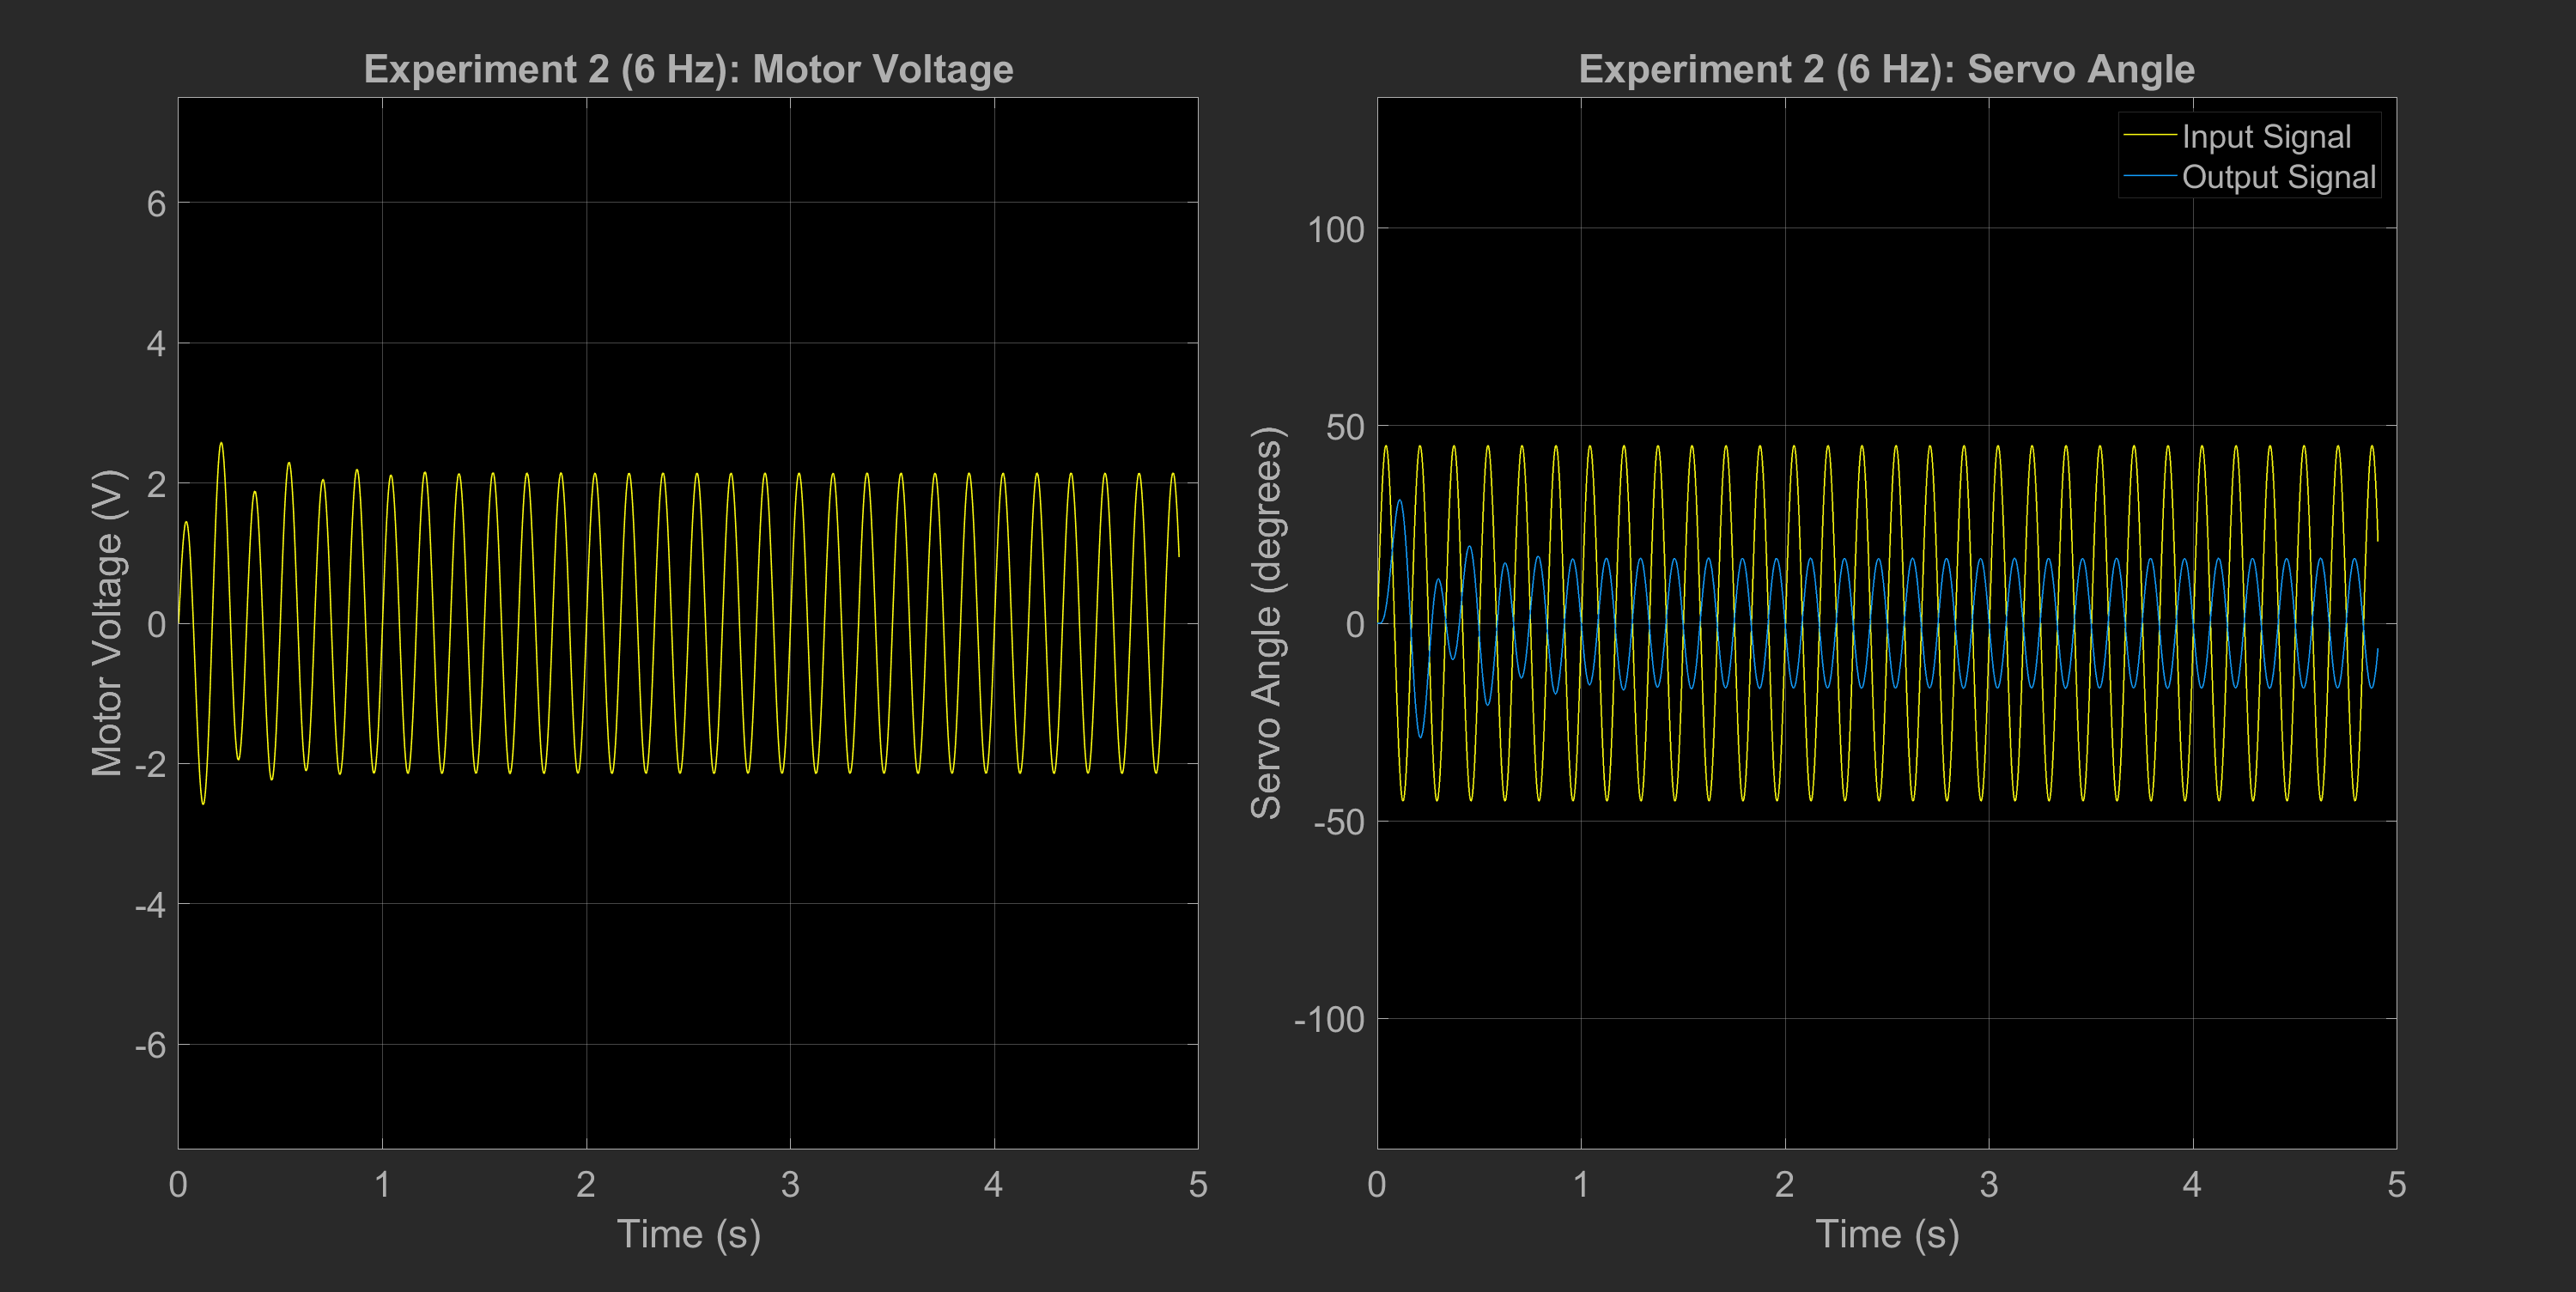
\includegraphics[width=0.87\textwidth]{exp2_6}
    \caption{\label{fig:exp2_6}Motor Voltage and Servo Angle for 6 Hz Input Signal}
\end{figure}

% general observations
In general, we can observe that the magnitude and phase of the output signal match our expectations based on Figure 3 from the lab document. There is no magnitude gain to start, with the gain beginning to increase until it reaches a peak value, then starts to decrease. There is no phase delay to start, with the delay beginning to increase then plateauing around 180 degrees.

% xiii) search for freq where mag reaches peak
To determine the frequency where the magnitude reaches its peak, we observed the change in the magnitude of the output signal using the "Peak Finder" tool as we changed the frequency. During our previous observations, the largest magnitude value occurred at 3 Hz. We determined the peak value by applying a binary search method beginning at 3 Hz, and eventually determined that the frequency where the magnitude reaches it peak value was around 3.06 Hz, where the magnitude was 139.9 degrees.


% xiv) use measurements to calculate motor parameters
We can use the recorded measurements to determine the value of the peak $M_p$ and the peak frequency $\omega_p$.
\begin{equation*}
\begin{aligned}[b]
    M_p &= \frac{139.9}{45} & \omega_p &= 2\pi3.06 \\
    &= 3.109 & &= 19.227
\end{aligned}
\end{equation*}
We can determine $\zeta$ and $\omega_n$ by using the equations derived in the prelab which relate them to $M_p$ and $\omega_p$.
\begin{equation*}
\begin{aligned}
    \zeta &= \sqrt{\frac{-4M_p^2 + \sqrt{14M_p^4 - 16M_p^2}}{-8M_p^2}} & \omega_n &= \frac{\omega_p}{\sqrt{1-2\zeta^2}} \\
    &= 0.163 & &= 19.759
\end{aligned}
\end{equation*}
We can determine the motor parameters $A$ and $\tau_m$ by using the equations derived in the prelab which relate them to $\zeta$ and $\omega_n$.
\begin{equation} \label{fig:exp2calc}
\begin{aligned}[b]
    A &= \frac{\omega_n / 2\zeta}{K} & \tau_m &= \frac{1}{2\omega_n\zeta} \\
    &= 30.303 & &= 0.155
\end{aligned}
\end{equation}
The values of $A$ and $\tau_m$ were determined to be 30.303 and 0.155 in Equation~\ref{fig:exp2calc}.

\clearpage
\section*{Comparison of Results and Discussion of Potential Discrepancies}
Our values for A and Tm were pretty close to each other using the 2 different methods. The discrepancies could've come from the non-linear effects of the motor or some shit xd.

\section*{Discussion on Improving the Accuracy of the Estimation of Model Parameters}
Who knows xd
Well for starters I think you'd want to reduce the non-linear effects of the motor as much as you could, so maybe you could increase the P-gain a little more.

\end{document}
